TODO: Išsiaiškinti ir suprasti. (Fizika12.png)

Magnetinis momentas:
\begin{equation*}
  \vec{p_{m}} = IS
\end{equation*}

\begin{figure}[H]
  \begin{center}
    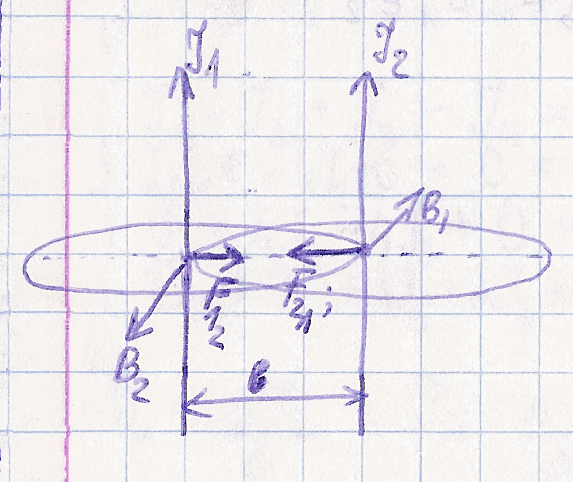
\includegraphics[height=0.5\textwidth]{images/bio_savaro_laplaso.png}
  \end{center}
  \caption{Bio-Savaro-Laplaso}
  \label{fig:bio_savaro_laplaso}
\end{figure}

\begin{defn}[Bio-Savaro-Laplaso dėsnis]
  Tarkime, kad turime du lygiagrečius begalinius laidininkus (žr.
  \ref{fig:bio_savaro_laplaso}), kuriais teka atitinkamai $I_{1}$
  ir $I_{2}$ stiprumo srovė, o tarp jų yra $b$ metrų tarpas.
  \begin{align*}
    \intertext{Tada pirmojo laidininko, antrojo laidininko taške,
    sukuriama indukcija bus lygi:}
    B_{1} &= \frac{\mu_{0}\mu 2 I_{1}}{4 \pi b} \\
    \intertext{Antrojo laidininko $dl$ ilgio atkarpą veiks jėga:}
    dF
    &= I_{2} \cdot B_{1} \cdot dl \\
    &= \frac{\mu_{0}\mu}{4 \pi} \frac{I_{1}\cdot I_{2}}{b} dl \\
  \end{align*}
  Gautoji išraiška vadinama Bio, Savaro, Laplaso dėsniu.
\end{defn}

TODO: Išsiaiškinti ir suprasti. (Fizika12.png)
TODO: Išsiaiškinti ir suprasti. (Fizika13.png)
